\section{微分中值定理}

\begin{problem}{多项式导数的实根分布}{Polynomial-Derivative-Real-Roots}
    设 $f(x) = (x-1)(x-2)(x-3)(x-4)$，确定方程 $f'(x) = 0$ 的实根的个数，并指出根所在的区间．
\end{problem}

\begin{solution}
    因为 $f(x)$ 为多项式函数，所以在 $\symbb{R}$ 上处处连续且可导．

    显然 $f(1) = f(2) = f(3) = f(4) = 0$．

    在区间 $[1, 2]$、$[2, 3]$ 及 $[3, 4]$ 上分别应用罗尔定理：
    \begin{enumerate}
        \item 由 $f(1) = f(2) = 0$，存在 $\xi_1 \in (1, 2)$，使得 $f'(\xi_1) = 0$；
        \item 由 $f(2) = f(3) = 0$，存在 $\xi_2 \in (2, 3)$，使得 $f'(\xi_2) = 0$；
        \item 由 $f(3) = f(4) = 0$，存在 $\xi_3 \in (3, 4)$，使得 $f'(\xi_3) = 0$．
    \end{enumerate}
    因为 $f(x)$ 是 $4$ 次多项式，其导数 $f'(x)$ 是 $3$ 次多项式，在复数域内至多有 $3$ 个根．

    因此方程 $f'(x) = 0$ 恰有 $3$ 个实根，分别位于区间 $(1, 2)$、$(2, 3)$ 和 $(3, 4)$ 内．
    \begin{equation}
        \boxed{\text{共有 } 3 \text{ 个实根，分别位于区间 } (1, 2)\text{、}(2, 3) \text{ 及 } (3, 4) \text{ 内．}}
    \end{equation}
\end{solution}

\begin{problem}{二阶导数零点的存在性证明}{Second-Derivative-Zero-Existence}
    设函数 $f(x)$ 在区间 $[1, 2]$ 上有二阶微商，且 $f(1) = f(2) = 0$．记 $F(x) = (x-1)^2 f(x)$，证明：在区间 $(1, 2)$ 内至少有一点 $\xi$，使得 $F''(\xi) = 0$．
\end{problem}

\begin{myproof}
    由题意，$F(x)$ 在区间 $[1, 2]$ 上具有二阶导数，且
    \begin{equation}
        F(1) = (1-1)^2 f(1) = 0, \qquad F(2) = (2-1)^2 f(2) = 0.
    \end{equation}
    由罗尔定理，存在 $\eta \in (1, 2)$，使得
    \begin{equation}
        F'(\eta) = 0.
    \end{equation}
    对 $F(x)$ 求导，得
    \begin{equation}
        F'(x) = 2(x-1)f(x) + (x-1)^2 f'(x) = (x-1)\bigl[ 2f(x) + (x-1)f'(x) \bigr].
    \end{equation}
    代入 $x = 1$，得
    \begin{equation}
        F'(1) = 0.
    \end{equation}
    因为 $F'(x)$ 在闭区间 $[1, \eta]$ 上连续，在开区间 $(1, \eta)$ 内可导，且 $F'(1) = F'(\eta) = 0$，由罗尔定理，存在 $\xi \in (1, \eta) \subset (1, 2)$，使得
    \begin{equation}
        F''(\xi) = 0.
    \end{equation}
\end{myproof}

\begin{problem}{微分中值定理逆命题的反例}{Counterexample-To-Converse-Of-MVT}
    举例说明，中值定理的下述意义下的逆不成立：设 $\xi \in (a, b)$ 是指定的一点，则存在 $c, d \in [a, b]$，使得 $\frac{f(c)-f(d)}{c-d} = f'(\xi)$．（提示：考虑函数 $f(x) = x^3$，$\xi = 0$．）
\end{problem}

\begin{solution}
    考虑闭区间 $[a, b] = [-1, 1]$ 上的函数 $f(x) = x^3$，并指定内点 $\xi = 0 \in (-1, 1)$．

    计算在 $\xi = 0$ 处的导数值：
    \begin{equation}
        f'(\xi) = f'(0) = \left. 3x^2 \right|_{x=0} = 0.
    \end{equation}
    若存在互不相同的点 $c, d \in [-1, 1]$（$c \neq d$），使得
    \begin{equation}
        \frac{f(c) - f(d)}{c - d} = f'(0) = 0,
    \end{equation}
    则有
    \begin{equation}
        \frac{c^3 - d^3}{c - d} = c^2 + cd + d^2 = \left( c + \frac{d}{2} \right)^2 + \frac{3}{4}d^2 = 0.
    \end{equation}
    因为各项均为非负实数，必有
    \begin{equation}
        c + \frac{d}{2} = 0 \quad \text{且} \quad d = 0 \implies c = d = 0,
    \end{equation}
    这与 $c \neq d$ 产生矛盾．

    因此不存在满足条件的 $c, d \in [-1, 1]$．
    \begin{equation}
        \boxed{f(x) = x^3, \quad x \in [-1, 1], \quad \xi = 0.}
    \end{equation}
\end{solution}

\begin{problem}{微分中值定理证明不等式}{Inequalities-Via-Mean-Value-Theorem}
    证明下列不等式：
    \begin{enumerate}
        \item 当 $a > b > 0, n > 1$ 时，有 $n b^{n-1}(a-b) < a^n - b^n < n a^{n-1}(a-b)$；
        \item 当 $x > 0$ 时，有 $\frac{x}{1+x} < \ln(1+x) < x$；
        \item 当 $0 < a < b$ 时，有 $(a+b)\ln \frac{a+b}{2} < a\ln a + b\ln b$；
        \item 当 $0 < \alpha < \beta < \frac{\uppi}{2}$ 时，有 $\frac{\beta-\alpha}{\cos^2 \alpha} < \tan \beta - \tan \alpha < \frac{\beta-\alpha}{\cos^2 \beta}$．
    \end{enumerate}
\end{problem}

\begin{myproof}
    \ansitem{1}

    对函数 $f(t) = t^n$ 在区间 $[b, a]$ 上应用拉格朗日中值定理，存在 $\xi \in (b, a)$，使得
    \begin{equation}
        a^n - b^n = n \xi^{n-1}(a - b).
    \end{equation}
    因为 $n > 1$ 且 $0 < b < \xi < a$，幂函数 $t^{n-1}$ 在 $(0, +\infty)$ 上严格单调递增，故
    \begin{equation}
        b^{n-1} < \xi^{n-1} < a^{n-1}.
    \end{equation}
    各边同乘以正数 $n(a - b) > 0$，即得
    \begin{equation}
        n b^{n-1}(a - b) < a^n - b^n < n a^{n-1}(a - b).
    \end{equation}

    \ansitem{2}

    对函数 $f(t) = \ln(1 + t)$ 在区间 $[0, x]$ 上应用拉格朗日中值定理，存在 $\xi \in (0, x)$，使得
    \begin{equation}
        \ln(1 + x) - \ln 1 = \frac{1}{1 + \xi} (x - 0) \implies \ln(1 + x) = \frac{x}{1 + \xi}.
    \end{equation}
    因为 $0 < \xi < x$，所以
    \begin{equation}
        \frac{1}{1 + x} < \frac{1}{1 + \xi} < 1.
    \end{equation}
    同乘以 $x > 0$，即得
    \begin{equation}
        \frac{x}{1 + x} < \ln(1 + x) < x.
    \end{equation}

    \ansitem{3}

    考虑函数 $f(t) = t\ln t$（$t > 0$）．其导数为 $f'(t) = \ln t + 1$，$f''(t) = \frac{1}{t} > 0$，故 $f(t)$ 为严格下凸函数．

    对区间 $[a, b]$ 应用琴生不等式（或中点凸性）：
    \begin{equation}
        f\left( \frac{a+b}{2} \right) < \frac{f(a) + f(b)}{2}.
    \end{equation}
    将 $f(t) = t\ln t$ 代入，得
    \begin{equation}
        \frac{a+b}{2} \ln \frac{a+b}{2} < \frac{a\ln a + b\ln b}{2}.
    \end{equation}
    两端同乘以 $2$，即得
    \begin{equation}
        (a+b)\ln \frac{a+b}{2} < a\ln a + b\ln b.
    \end{equation}

    \ansitem{4}

    对函数 $f(t) = \tan t$ 在区间 $[\alpha, \beta] \subset \left(0, \frac{\uppi}{2}\right)$ 上应用拉格朗日中值定理，存在 $\xi \in (\alpha, \beta)$，使得
    \begin{equation}
        \tan \beta - \tan \alpha = \sec^2 \xi (\beta - \alpha) = \frac{\beta - \alpha}{\cos^2 \xi}.
    \end{equation}
    因为余弦函数在 $\left(0, \frac{\uppi}{2}\right)$ 内严格单调递减，由 $0 < \alpha < \xi < \beta < \frac{\uppi}{2}$ 可知
    \begin{equation}
        0 < \cos \beta < \cos \xi < \cos \alpha \implies \frac{1}{\cos^2 \alpha} < \frac{1}{\cos^2 \xi} < \frac{1}{\cos^2 \beta}.
    \end{equation}
    各边同乘以正数 $\beta - \alpha > 0$，即得
    \begin{equation}
        \frac{\beta - \alpha}{\cos^2 \alpha} < \tan \beta - \tan \alpha < \frac{\beta - \alpha}{\cos^2 \beta}.
    \end{equation}
\end{myproof}

\begin{problem}{导数为零证明反三角恒等式}{Inverse-Trigonometric-Identities-Proof}
    证明下列恒等式：
    \begin{enumerate}
        \item $\arctan x = \arcsin \frac{x}{\sqrt{1+x^2}}$；
        \item $\arctan x + \arctan \frac{1-x}{1+x} = \begin{cases} \frac{\uppi}{4}, & x > -1, \\ -\frac{3\uppi}{4}, & x < -1. \end{cases}$
    \end{enumerate}
\end{problem}

\begin{myproof}
    \ansitem{1}

    令函数 $f(x) = \arcsin \frac{x}{\sqrt{1+x^2}} - \arctan x$（$x \in \symbb{R}$）．求导得
    \begin{equation}
        \begin{aligned}
            f'(x) & = \frac{1}{\sqrt{1 - \frac{x^2}{1+x^2}}} \cdot \frac{\sqrt{1+x^2} - x \cdot \frac{x}{\sqrt{1+x^2}}}{1+x^2} - \frac{1}{1+x^2} \\
                  & = \sqrt{1+x^2} \cdot \frac{1}{(1+x^2)^{3/2}} - \frac{1}{1+x^2}                                                               \\
                  & = \frac{1}{1+x^2} - \frac{1}{1+x^2} = 0.
        \end{aligned}
    \end{equation}
    故 $f(x) \equiv C$（常数）．代入 $x = 0$，有
    \begin{equation}
        C = f(0) = \arcsin 0 - \arctan 0 = 0.
    \end{equation}
    因此 $\arctan x = \arcsin \frac{x}{\sqrt{1+x^2}}$ 对一切 $x \in \symbb{R}$ 恒成立．

    \ansitem{2}

    令函数 $g(x) = \arctan x + \arctan \frac{1-x}{1+x}$（$x \neq -1$）．求导得
    \begin{equation}
        \begin{aligned}
            g'(x) & = \frac{1}{1+x^2} + \frac{1}{1 + \left(\frac{1-x}{1+x}\right)^2} \cdot \frac{-(1+x) - (1-x)}{(1+x)^2} \\
                  & = \frac{1}{1+x^2} + \frac{-2}{(1+x)^2 + (1-x)^2}                                                      \\
                  & = \frac{1}{1+x^2} - \frac{2}{2(1+x^2)} = 0.
        \end{aligned}
    \end{equation}
    在区间 $(-1, +\infty)$ 上，$g'(x) = 0 \implies g(x) \equiv C_1$．代入 $x = 0$，得
    \begin{equation}
        C_1 = g(0) = \arctan 0 + \arctan 1 = \frac{\uppi}{4}.
    \end{equation}
    在区间 $(-\infty, -1)$ 上，$g'(x) = 0 \implies g(x) \equiv C_2$．取 $x \to -\infty$ 计算极限：
    \begin{equation}
        C_2 = \lim_{x\to -\infty} g(x) = \left( -\frac{\uppi}{2} \right) + \arctan(-1) = -\frac{\uppi}{2} - \frac{\uppi}{4} = -\frac{3\uppi}{4}.
    \end{equation}
    综上，原恒等式得证．
\end{myproof}

\begin{problem}{导数非一函数的不动点唯一性}{Unique-Fixed-Point-Theorem}
    设 $f(x)$ 是闭区间 $[0, 1]$ 上的可导函数，对任意 $x \in [0, 1]$ 有 $f(x) \in (0, 1)$；并且对每个 $x$，$f'(x) \neq 1$．证明：在 $(0, 1)$ 内有且仅有一个 $x$，使 $f(x) = x$．
\end{problem}

\begin{myproof}
    令辅助函数 $g(x) = f(x) - x$．因 $f(x)$ 可导，故 $g(x)$ 在 $[0, 1]$ 上连续．

    考察端点处的函数值：由 $f(x) \in (0, 1)$ 可知
    \begin{equation}
        g(0) = f(0) - 0 = f(0) > 0,
    \end{equation}
    \begin{equation}
        g(1) = f(1) - 1 < 0.
    \end{equation}
    由零点存在定理，存在 $x_0 \in (0, 1)$，使得 $g(x_0) = 0$，即 $f(x_0) = x_0$．

    再证唯一性：采用反证法．若在 $(0, 1)$ 内存在两个互不相同的点 $x_1 < x_2$，满足 $f(x_1) = x_1$ 且 $f(x_2) = x_2$．

    此时 $g(x_1) = g(x_2) = 0$．由罗尔定理，存在 $\xi \in (x_1, x_2) \subset (0, 1)$，使得
    \begin{equation}
        g'(\xi) = 0 \implies f'(\xi) - 1 = 0 \implies f'(\xi) = 1,
    \end{equation}
    这与已知条件“对每个 $x$ 恒有 $f'(x) \neq 1$”矛盾．

    故在 $(0, 1)$ 内有且仅有一个 $x$ 满足 $f(x) = x$．
\end{myproof}

\begin{problem}{导数有界与端点相等的函数值震荡估计}{Oscillation-Estimation-Via-Bounded-Derivative}
    设函数 $f(x)$ 在 $[0, 1]$ 上连续，在 $(0, 1)$ 内可导，且 $|f'(x)| < 1$，又 $f(0) = f(1)$．证明：对于 $[0, 1]$ 上的任意两点 $x_1, x_2$，有 $|f(x_1) - f(x_2)| < \frac{1}{2}$．
\end{problem}

\begin{myproof}
    不妨设 $0 \leqslant x_1 < x_2 \leqslant 1$．
    \begin{enumerate}
        \item 若 $x_2 - x_1 \leqslant \frac{1}{2}$：在区间 $[x_1, x_2]$ 上应用拉格朗日中值定理，存在 $\xi \in (x_1, x_2)$，使得
              \begin{equation}
                  |f(x_1) - f(x_2)| = |f'(\xi)| (x_2 - x_1) < 1 \cdot (x_2 - x_1) \leqslant \frac{1}{2};
              \end{equation}
        \item 若 $x_2 - x_1 > \frac{1}{2}$：利用 $f(0) = f(1)$，作恒等变形：
              \begin{equation}
                  f(x_2) - f(x_1) = \bigl[ f(x_2) - f(1) \bigr] + \bigl[ f(0) - f(x_1) \bigr].
              \end{equation}
              分别在 $[x_2, 1]$ 与 $[0, x_1]$ 上应用拉格朗日中值定理，存在 $\xi_1 \in (x_2, 1)$ 和 $\xi_2 \in (0, x_1)$，得
              \begin{equation}
                  \begin{aligned}
                      |f(x_1) - f(x_2)| & \leqslant |f(1) - f(x_2)| + |f(x_1) - f(0)|        \\
                                        & = |f'(\xi_1)|(1 - x_2) + |f'(\xi_2)|(x_1 - 0)      \\
                                        & < 1 \cdot (1 - x_2) + 1 \cdot x_1                  \\
                                        & = 1 - (x_2 - x_1) < 1 - \frac{1}{2} = \frac{1}{2}.
                  \end{aligned}
              \end{equation}
    \end{enumerate}
    综上，对 $[0, 1]$ 上的任意两点 $x_1, x_2$，恒有 $|f(x_1) - f(x_2)| < \frac{1}{2}$．
\end{myproof}

\begin{problem}{常微分方程 $f'=f$ 的解的结构}{Differential-Equation-F-Prime-Equals-F}
    若 $f(x)$ 处处可导，且 $f'(x) = f(x)$．证明：$f(x) = C\e^x$，$C$ 为任意常数．
\end{problem}

\begin{myproof}
    构造辅助函数
    \begin{equation}
        g(x) = f(x)\e^{-x}, \quad x \in \symbb{R}.
    \end{equation}
    因 $f(x)$ 与 $\e^{-x}$ 在 $\symbb{R}$ 上处处可导，对 $g(x)$ 求导得
    \begin{equation}
        g'(x) = f'(x)\e^{-x} - f(x)\e^{-x} = \bigl[ f'(x) - f(x) \bigr]\e^{-x}.
    \end{equation}
    由已知条件 $f'(x) = f(x)$，得
    \begin{equation}
        g'(x) = 0 \cdot \e^{-x} = 0.
    \end{equation}
    因为在区间 $(-\infty, +\infty)$ 上导数处处为零，所以 $g(x)$ 必为常数函数，即存在常数 $C$ 使得
    \begin{equation}
        g(x) \equiv C \implies f(x)\e^{-x} = C \implies f(x) = C\e^x.
    \end{equation}
\end{myproof}

\begin{problem}{非常值函数正导数值点的存在性}{Existence-Of-Positive-Derivative-Point}
    设不恒为常数的函数 $f(x)$ 在闭区间 $[a, b]$ 上连续，在开区间 $(a, b)$ 内可导，且 $f(a) = f(b)$．证明：在 $(a, b)$ 内存在一点 $\xi$，使得 $f'(\xi) > 0$．
\end{problem}

\begin{myproof}
    因为 $f(x)$ 在闭区间 $[a, b]$ 上连续，由最大值最小值定理，$f(x)$ 在 $[a, b]$ 上取得最大值 $M$ 与最小值 $m$．

    由于 $f(x)$ 不恒为常数，必有 $m < M$．故 $M$ 与 $m$ 中至少有一个不等于端点值 $f(a) = f(b)$：
    \begin{enumerate}
        \item 若 $M > f(a)$：最大值在内点 $x_0 \in (a, b)$ 处取得，即 $f(x_0) = M > f(a)$．在区间 $[a, x_0]$ 上应用拉格朗日中值定理，存在 $\xi \in (a, x_0) \subset (a, b)$，使得
              \begin{equation}
                  f'(\xi) = \frac{f(x_0) - f(a)}{x_0 - a} > 0;
              \end{equation}
        \item 若 $m < f(a)$：最小值在内点 $x_1 \in (a, b)$ 处取得，即 $f(x_1) = m < f(b)$．在区间 $[x_1, b]$ 上应用拉格朗日中值定理，存在 $\xi \in (x_1, b) \subset (a, b)$，使得
              \begin{equation}
                  f'(\xi) = \frac{f(b) - f(x_1)}{b - x_1} > 0.
              \end{equation}
    \end{enumerate}
    综上，在 $(a, b)$ 内必存在一点 $\xi$，使得 $f'(\xi) > 0$．
\end{myproof}

\begin{problem}{导数趋于零的渐近性质}{Asymptotic-Behavior-With-Vanishing-Derivative}
    设函数 $f(x)$ 在 $[a, +\infty)$ 上可微，且 $\lim_{x\to +\infty} f'(x) = 0$．证明：
    \begin{enumerate}
        \item $\lim_{x\to +\infty} [f(x+1) - f(x)] = 0$；
        \item $\lim_{x\to +\infty} \frac{f(x)}{x} = 0$．
    \end{enumerate}
\end{problem}

\begin{myproof}
    \ansitem{1}

    对任意 $x \geqslant a$，在闭区间 $[x, x+1]$ 上应用拉格朗日中值定理，存在 $\xi_x \in (x, x+1)$，使得
    \begin{equation}
        f(x+1) - f(x) = f'(\xi_x)(x+1 - x) = f'(\xi_x).
    \end{equation}
    当 $x \to +\infty$ 时，因为 $\xi_x > x$，所以 $\xi_x \to +\infty$．由已知 $\lim_{t\to +\infty} f'(t) = 0$，有
    \begin{equation}
        \lim_{x\to +\infty} [f(x+1) - f(x)] = \lim_{x\to +\infty} f'(\xi_x) = 0.
    \end{equation}

    \ansitem{2}

    对任给 $\varepsilon > 0$，由 $\lim_{t\to +\infty} f'(t) = 0$，存在实数 $X > \max\{a, 0\}$，使得当 $t > X$ 时，恒有
    \begin{equation}
        |f'(t)| < \frac{\varepsilon}{2}.
    \end{equation}
    对任意 $x > X$，在区间 $[X, x]$ 上应用拉格朗日中值定理，存在 $\xi \in (X, x)$，使得
    \begin{equation}
        f(x) - f(X) = f'(\xi)(x - X) \implies \frac{f(x)}{x} = \frac{f(X)}{x} + f'(\xi)\left( 1 - \frac{X}{x} \right).
    \end{equation}
    由于 $0 < 1 - \frac{X}{x} < 1$ 且 $\xi > X$，利用绝对值三角不等式，有
    \begin{equation}
        \left| \frac{f(x)}{x} \right| \leqslant \frac{|f(X)|}{x} + |f'(\xi)| < \frac{|f(X)|}{x} + \frac{\varepsilon}{2}.
    \end{equation}
    因为 $X$ 为定值，$\lim_{x\to +\infty} \frac{|f(X)|}{x} = 0$，故存在 $X' > X$，使得当 $x > X'$ 时，有 $\frac{|f(X)|}{x} < \frac{\varepsilon}{2}$．

    从而当 $x > X'$ 时，恒有
    \begin{equation}
        \left| \frac{f(x)}{x} \right| < \frac{\varepsilon}{2} + \frac{\varepsilon}{2} = \varepsilon.
    \end{equation}
    由极限定义，即得 $\lim_{x\to +\infty} \frac{f(x)}{x} = 0$．
\end{myproof}

\begin{problem}{导函数有界性与函数有界性的关系}{Bounded-Derivative-And-Function-Boundedness}
    证明：若函数 $f(x)$ 在（有限）开区间 $(a, b)$ 内有有界的导函数，则 $f(x)$ 在 $(a, b)$ 内也有界．如果有限区间 $(a, b)$ 改为无穷区间，结论还成立吗？命题的逆命题是否成立？
\end{problem}

\begin{solution}
    先证充分性：

    设导函数在有限开区间 $(a, b)$ 内有界，即存在常数 $M > 0$，使得对任意 $t \in (a, b)$ 均有 $|f'(t)| \leqslant M$．

    取定一点 $x_0 \in (a, b)$．对区间 $(a, b)$ 内的任意点 $x$，由拉格朗日中值定理，存在 $\xi$ 介于 $x$ 与 $x_0$ 之间，使得
    \begin{equation}
        f(x) - f(x_0) = f'(\xi)(x - x_0).
    \end{equation}
    应用绝对值不等式：
    \begin{equation}
        |f(x)| \leqslant |f(x_0)| + |f'(\xi)| |x - x_0| \leqslant |f(x_0)| + M(b - a).
    \end{equation}
    因为 $|f(x_0)| + M(b - a)$ 是与 $x$ 无关的有限常数，所以 $f(x)$ 在 $(a, b)$ 内有界．

    对于无穷区间，结论不成立：

    例如在无穷区间 $(0, +\infty)$ 上，函数 $f(x) = x$ 的导函数为 $f'(x) = 1$，显然有界，但函数 $f(x) = x$ 在 $(0, +\infty)$ 上无界．

    逆命题不成立：

    反例：在有限开区间 $(0, 1)$ 上，函数 $f(x) = \sqrt{x}$ 有界（$0 < f(x) < 1$），但其导函数 $f'(x) = \frac{1}{2\sqrt{x}}$ 在 $(0, 1)$ 上无界（当 $x \to 0^+$ 时 $f'(x) \to +\infty$）．
    \begin{equation}
        \boxed{\text{无穷区间上结论不成立；逆命题不成立．}}
    \end{equation}
\end{solution}

\begin{problem}{高阶利普希茨条件下的函数性质}{Higher-Order-Lipschitz-Condition}
    设对所有的实数 $x, y$，不等式 $|f(x) - f(y)| \leqslant M|x - y|^2$（$M$ 为常数）都成立．证明：$f(x)$ 恒为常数．
\end{problem}

\begin{myproof}
    任取 $x \in \symbb{R}$．对任意 $h \neq 0$，由题设不等式，有
    \begin{equation}
        |f(x+h) - f(x)| \leqslant M |(x+h) - x|^2 = M h^2.
    \end{equation}
    两端同除以 $|h| > 0$，得
    \begin{equation}
        0 \leqslant \left| \frac{f(x+h) - f(x)}{h} \right| \leqslant M|h|.
    \end{equation}
    因为 $\lim_{h\to 0} M|h| = 0$，由夹逼准则可得
    \begin{equation}
        f'(x) = \lim_{h\to 0} \frac{f(x+h) - f(x)}{h} = 0.
    \end{equation}
    由于导数 $f'(x) = 0$ 对任意 $x \in \symbb{R}$ 恒成立，由拉格朗日中值定理推论，函数 $f(x)$ 在 $\symbb{R}$ 上恒为常数．
\end{myproof}

\begin{problem}{导数符号与严格单调性}{Derivative-Sign-And-Strict-Monotonicity}
    设 $f(x)$ 在一个区间 $I$ 上连续，且（至多）除了有限个点外，$f(x)$ 在 $I$ 内部的导数为正（负），证明：$f(x)$ 在 $I$ 上严格单调递增（减）．（注意，在例外的点处，$f(x)$ 可能不可导．）
\end{problem}

\begin{myproof}
    以导数为正的情形为例进行证明（导数为负的情形完全对称）．

    任取 $x_1, x_2 \in I$ 且 $x_1 < x_2$．闭区间 $[x_1, x_2]$ 内至多包含有限个例外点，记为 $c_1 < c_2 < \cdots < c_k$．

    将区间 $[x_1, x_2]$ 划分为有限个子区间 $[t_{j-1}, t_j]$（$j = 1, 2, \cdots, m$），满足
    \begin{equation}
        x_1 = t_0 < t_1 < t_2 < \cdots < t_m = x_2,
    \end{equation}
    且每个开区间 $(t_{j-1}, t_j)$ 内部均不包含任何例外点．

    在每个子区间 $[t_{j-1}, t_j]$ 上，函数 $f(x)$ 连续，且在 $(t_{j-1}, t_j)$ 内可导并满足 $f'(x) > 0$．由拉格朗日中值定理，存在 $\xi_j \in (t_{j-1}, t_j)$，使得
    \begin{equation}
        f(t_j) - f(t_{j-1}) = f'(\xi_j)(t_j - t_{j-1}).
    \end{equation}
    因为 $f'(\xi_j) > 0$ 且 $t_j - t_{j-1} > 0$，所以
    \begin{equation}
        f(t_j) - f(t_{j-1}) > 0 \quad (j = 1, 2, \cdots, m).
    \end{equation}
    将上述 $m$ 个正不等式逐项累加，得
    \begin{equation}
        f(x_2) - f(x_1) = \sum_{j=1}^m \bigl[ f(t_j) - f(t_{j-1}) \bigr] > 0 \implies f(x_1) < f(x_2).
    \end{equation}
    由 $x_1 < x_2$ 的任意性，可知 $f(x)$ 在区间 $I$ 上严格单调递增．
\end{myproof}

\begin{problem}{导数大小比较与函数值不等式}{Derivative-Comparison-And-Function-Inequality}
    设函数 $f(x)$ 和 $g(x)$ 均在区间 $I$ 上连续，且（至多）除了有限个点外，$f(x)$ 和 $g(x)$ 在 $I$ 内部满足 $f'(x) > g'(x)$；设存在 $a \in I$，使得 $f(a) = g(a)$（$a$ 不是区间端点），证明：当 $x \in I$ 且 $x > a$ 时，有 $f(x) > g(x)$；当 $x \in I$ 且 $x < a$ 时，有 $f(x) < g(x)$．
\end{problem}

\begin{myproof}
    构造辅助函数
    \begin{equation}
        h(x) = f(x) - g(x), \quad x \in I.
    \end{equation}
    因为 $f(x)$ 与 $g(x)$ 在区间 $I$ 上连续，所以 $h(x)$ 在区间 $I$ 上连续．

    在区间 $I$ 内部，除至多有限个点外，恒有
    \begin{equation}
        h'(x) = f'(x) - g'(x) > 0.
    \end{equation}
    由严格单调性判定定理，函数 $h(x)$ 在区间 $I$ 上严格单调递增．

    又因为 $h(a) = f(a) - g(a) = 0$，由严格单调递增性可得：
    \begin{enumerate}
        \item 当 $x \in I$ 且 $x > a$ 时，$h(x) > h(a) = 0 \implies f(x) > g(x)$；
        \item 当 $x \in I$ 且 $x < a$ 时，$h(x) < h(a) = 0 \implies f(x) < g(x)$．
    \end{enumerate}
    命题得证．
\end{myproof}

\begin{problem}{斜率函数的严格单调性}{Strict-Monotonicity-Of-Secant-Slope}
    若 $f(x)$ 在 $[0, +\infty)$ 可导，$f(0) = 0$，$f'(x)$ 严格递增，证明：$\frac{f(x)}{x}$ 在 $(0, +\infty)$ 内严格递增．
\end{problem}

\begin{myproof}
    令辅助函数
    \begin{equation}
        g(x) = \frac{f(x)}{x}, \quad x \in (0, +\infty).
    \end{equation}
    对 $g(x)$ 求导，得
    \begin{equation}
        g'(x) = \frac{x f'(x) - f(x)}{x^2}.
    \end{equation}
    对任意 $x > 0$，函数 $f(t)$ 在闭区间 $[0, x]$ 上连续，在开区间 $(0, x)$ 内可导．由拉格朗日中值定理及 $f(0) = 0$，存在 $\xi \in (0, x)$，使得
    \begin{equation}
        f(x) = f(x) - f(0) = f'(\xi)x.
    \end{equation}
    将上式代入导数表达式中，得
    \begin{equation}
        g'(x) = \frac{x f'(x) - x f'(\xi)}{x^2} = \frac{f'(x) - f'(\xi)}{x}.
    \end{equation}
    因为 $f'(x)$ 在 $[0, +\infty)$ 上严格单调递增，且 $0 < \xi < x$，所以
    \begin{equation}
        f'(x) - f'(\xi) > 0.
    \end{equation}
    结合 $x > 0$，可知对任意 $x \in (0, +\infty)$ 恒有
    \begin{equation}
        g'(x) > 0.
    \end{equation}
    故函数 $g(x) = \frac{f(x)}{x}$ 在 $(0, +\infty)$ 内严格单调递增．
\end{myproof}

\begin{problem}{二阶导数极值判别法与反例}{Second-Derivative-Test-And-Examples}
    设 $x_0$ 是函数 $f(x)$ 的一个驻点（$f'(x_0) = 0$），且 $f(x)$ 在 $x_0$ 处二阶可微，$f''(x_0) \neq 0$．证明：若 $f''(x_0) < 0$，则 $x_0$ 是 $f(x)$ 的一个极大值点；若 $f''(x_0) > 0$，则 $x_0$ 是 $f(x)$ 的一个极小值点．
    举例说明：若 $f''(x_0) = 0$，则 $x_0$ 可以是 $f(x)$ 的极大值点或极小值点，也可以不是极值点．
\end{problem}

\begin{solution}
    将 $f(x)$ 在点 $x_0$ 处展开为带佩亚诺余项的泰勒公式：
    \begin{equation}
        f(x) = f(x_0) + f'(x_0)(x - x_0) + \frac{1}{2}f''(x_0)(x - x_0)^2 + o\bigl((x - x_0)^2\bigr).
    \end{equation}
    将驻点条件 $f'(x_0) = 0$ 代入，得
    \begin{equation}
        f(x) - f(x_0) = \frac{1}{2}(x - x_0)^2 \left[ f''(x_0) + \alpha(x) \right],
    \end{equation}
    其中 $\lim_{x\to x_0} \alpha(x) = 0$．

    若 $f''(x_0) < 0$，取 $\varepsilon = \frac{|f''(x_0)|}{2} > 0$，存在 $\delta > 0$，使得当 $0 < |x - x_0| < \delta$ 时，有 $|\alpha(x)| < \frac{|f''(x_0)|}{2}$，从而
    \begin{equation}
        f''(x_0) + \alpha(x) < \frac{1}{2}f''(x_0) < 0.
    \end{equation}
    故当 $0 < |x - x_0| < \delta$ 时，$f(x) - f(x_0) < 0 \implies f(x) < f(x_0)$，点 $x_0$ 为 $f(x)$ 的严格极大值点．

    若 $f''(x_0) > 0$，同理可得在去心邻域内 $f''(x_0) + \alpha(x) > 0$，从而 $f(x) > f(x_0)$，点 $x_0$ 为 $f(x)$ 的严格极小值点．

    当 $f''(x_0) = 0$ 时的反例如下（均取 $x_0 = 0$）：
    \begin{enumerate}
        \item 极小值点：$f(x) = x^4$，此时 $f'(0) = 0$，$f''(0) = 0$，但对任意 $x \neq 0$ 恒有 $f(x) > 0 = f(0)$，故 $x = 0$ 为极小值点；
        \item 极大值点：$f(x) = -x^4$，此时 $f'(0) = 0$，$f''(0) = 0$，但对任意 $x \neq 0$ 恒有 $f(x) < 0 = f(0)$，故 $x = 0$ 为极大值点；
        \item 非极值点：$f(x) = x^3$，此时 $f'(0) = 0$，$f''(0) = 0$，但函数在实轴上严格单调递增，$x = 0$ 为拐点而非极值点．
    \end{enumerate}
    \begin{equation}
        \boxed{\text{极小值例：} f(x) = x^4；\text{极大值例：} f(x) = -x^4；\text{非极值例：} f(x) = x^3．}
    \end{equation}
\end{solution}

\begin{problem}{罗尔定理与二阶导数方程}{Second-Derivative-Rolle-Theorem}
    设 $f(x)$ 在 $[0, 1]$ 上有二阶导函数，且 $f(0) = f'(0)$，$f(1) = f'(1)$．求证：存在 $\xi \in (0, 1)$，满足 $f(\xi) = f''(\xi)$．
\end{problem}

\begin{myproof}
    构造辅助函数
    \begin{equation}
        F(x) = \e^x \bigl[ f(x) - f'(x) \bigr], \quad x \in [0, 1].
    \end{equation}
    因为 $f(x)$ 在 $[0, 1]$ 上具有二阶导函数，所以 $F(x)$ 在 $[0, 1]$ 上连续，在 $(0, 1)$ 内可导．

    计算两端点处的函数值：
    \begin{equation}
        F(0) = \e^0 \bigl[ f(0) - f'(0) \bigr] = 1 \cdot 0 = 0,
    \end{equation}
    \begin{equation}
        F(1) = \e^1 \bigl[ f(1) - f'(1) \bigr] = \e \cdot 0 = 0.
    \end{equation}
    对 $F(x)$ 求导，得
    \begin{equation}
        \begin{aligned}
            F'(x) & = \e^x \bigl[ f(x) - f'(x) \bigr] + \e^x \bigl[ f'(x) - f''(x) \bigr] \\
                  & = \e^x \bigl[ f(x) - f''(x) \bigr].
        \end{aligned}
    \end{equation}
    因为 $F(0) = F(1) = 0$，由罗尔定理，在开区间 $(0, 1)$ 内至少存在一点 $\xi$，使得
    \begin{equation}
        F'(\xi) = 0 \implies \e^\xi \bigl[ f(\xi) - f''(\xi) \bigr] = 0.
    \end{equation}
    由于指数函数 $\e^\xi \neq 0$，两边同除以 $\e^\xi$，即得
    \begin{equation}
        f(\xi) = f''(\xi).
    \end{equation}
\end{myproof}

\begin{problem}{函数单调区间与极值的求解}{Monotonicity-Intervals-And-Extrema}
    求下列函数的单调区间与极值：
    \begin{enumerate}
        \item $y = 2x^3 - 3x^2$；
        \item $y = x^{2/3}$；
        \item $y = x^2 \e^{-x^2}$；
        \item $y = x^{1/x}$；
        \item $y = \frac{(\ln x)^2}{x}$；
        \item $y = \arctan x - \frac{1}{2}\ln(1 + x^2)$．
    \end{enumerate}
\end{problem}

\begin{solution}
    \ansitem{1}

    求导得 $y' = 6x^2 - 6x = 6x(x - 1)$．驻点为 $x = 0, 1$．
    \begin{enumerate}
        \item 当 $x \in (-\infty, 0)$ 时，$y' > 0$，函数严格单调递增；
        \item 当 $x \in (0, 1)$ 时，$y' < 0$，函数严格单调递减；
        \item 当 $x \in (1, +\infty)$ 时，$y' > 0$，函数严格单调递增．
    \end{enumerate}
    极大值为 $y(0) = 0$；极小值为 $y(1) = -1$．
    \begin{equation}
        \boxed{
        \begin{aligned}
             & \text{单调递增区间：} (-\infty, 0]\text{、}[1, +\infty)\text{；单调递减区间：} [0, 1]\text{；} \\
             & \text{极大值：} y(0) = 0\text{；极小值：} y(1) = -1.
        \end{aligned}
        }
    \end{equation}

    \ansitem{2}

    当 $x \neq 0$ 时，求导得 $y' = \frac{2}{3x^{1/3}}$．
    \begin{enumerate}
        \item 当 $x \in (-\infty, 0)$ 时，$y' < 0$，函数严格单调递减；
        \item 当 $x \in (0, +\infty)$ 时，$y' > 0$，函数严格单调递增．
    \end{enumerate}
    在 $x = 0$ 处导数不存在，极小值为 $y(0) = 0$；无极大值．
    \begin{equation}
        \boxed{
        \begin{aligned}
             & \text{单调递减区间：} (-\infty, 0]\text{；单调递增区间：} [0, +\infty)\text{；} \\
             & \text{极小值：} y(0) = 0\text{；无极大值．}
        \end{aligned}
        }
    \end{equation}

    \ansitem{3}

    求导得 $y' = 2x(1 - x^2)\e^{-x^2} = -2x(x - 1)(x + 1)\e^{-x^2}$．驻点为 $x = -1, 0, 1$．
    \begin{enumerate}
        \item 当 $x \in (-\infty, -1)$ 时，$y' > 0$，函数严格单调递增；
        \item 当 $x \in (-1, 0)$ 时，$y' < 0$，函数严格单调递减；
        \item 当 $x \in (0, 1)$ 时，$y' > 0$，函数严格单调递增；
        \item 当 $x \in (1, +\infty)$ 时，$y' < 0$，函数严格单调递减．
    \end{enumerate}
    极大值为 $y(\pm 1) = \frac{1}{\e}$；极小值为 $y(0) = 0$．
    \begin{equation}
        \boxed{
        \begin{aligned}
             & \text{单调递增区间：} (-\infty, -1]\text{、}[0, 1]\text{；单调递减区间：} [-1, 0]\text{、}[1, +\infty)\text{；} \\
             & \text{极大值：} y(-1) = y(1) = \frac{1}{\e}\text{；极小值：} y(0) = 0.
        \end{aligned}
        }
    \end{equation}

    \ansitem{4}

    定义域为 $(0, +\infty)$．求导得 $y' = x^{1/x} \frac{1 - \ln x}{x^2}$．驻点为 $x = \e$．
    \begin{enumerate}
        \item 当 $x \in (0, \e)$ 时，$y' > 0$，函数严格单调递增；
        \item 当 $x \in (\e, +\infty)$ 时，$y' < 0$，函数严格单调递减．
    \end{enumerate}
    极大值为 $y(\e) = \e^{1/\e}$；无极小值．
    \begin{equation}
        \boxed{
        \begin{aligned}
             & \text{单调递增区间：} (0, \e]\text{；单调递减区间：} [\e, +\infty)\text{；} \\
             & \text{极大值：} y(\e) = \e^{1/\e}\text{；无极小值．}
        \end{aligned}
        }
    \end{equation}

    \ansitem{5}

    定义域为 $(0, +\infty)$．求导得 $y' = \frac{\ln x(2 - \ln x)}{x^2}$．驻点为 $x = 1, \e^2$．
    \begin{enumerate}
        \item 当 $x \in (0, 1)$ 时，$y' < 0$，函数严格单调递减；
        \item 当 $x \in (1, \e^2)$ 时，$y' > 0$，函数严格单调递增；
        \item 当 $x \in (\e^2, +\infty)$ 时，$y' < 0$，函数严格单调递减．
    \end{enumerate}
    极小值为 $y(1) = 0$；极大值为 $y(\e^2) = \frac{4}{\e^2}$．
    \begin{equation}
        \boxed{
        \begin{aligned}
             & \text{单调递减区间：} (0, 1]\text{、}[\e^2, +\infty)\text{；单调递增区间：} [1, \e^2]\text{；} \\
             & \text{极小值：} y(1) = 0\text{；极大值：} y(\e^2) = \frac{4}{\e^2}.
        \end{aligned}
        }
    \end{equation}

    \ansitem{6}

    定义域为 $\symbb{R}$．求导得 $y' = \frac{1}{1+x^2} - \frac{x}{1+x^2} = \frac{1 - x}{1+x^2}$．驻点为 $x = 1$．
    \begin{enumerate}
        \item 当 $x \in (-\infty, 1)$ 时，$y' > 0$，函数严格单调递增；
        \item 当 $x \in (1, +\infty)$ 时，$y' < 0$，函数严格单调递减．
    \end{enumerate}
    极大值为 $y(1) = \frac{\uppi}{4} - \frac{1}{2}\ln 2$；无极小值．
    \begin{equation}
        \boxed{
        \begin{aligned}
             & \text{单调递增区间：} (-\infty, 1]\text{；单调递减区间：} [1, +\infty)\text{；}    \\
             & \text{极大值：} y(1) = \frac{\uppi}{4} - \frac{1}{2}\ln 2\text{；无极小值．}
        \end{aligned}
        }
    \end{equation}
\end{solution}

\begin{problem}{区间上函数的最值求解}{Extreme-Values-On-Intervals}
    求下列函数在所给区间上的最大值和最小值：
    \begin{enumerate}
        \item $y = x^4 - 2x^2 + 5$，$x \in [-2, 2]$；
        \item $y = \sin 2x - x$，$x \in \left[-\frac{\uppi}{2}, \frac{\uppi}{2}\right]$；
        \item $y = \arctan \frac{1-x}{1+x}$，$x \in [0, 1]$；
        \item $y = x \ln x$，$x \in (0, +\infty)$．
    \end{enumerate}
\end{problem}

\begin{solution}
    \ansitem{1}

    求导得 $y' = 4x^3 - 4x = 4x(x - 1)(x + 1)$．

    在区间 $[-2, 2]$ 内的驻点为 $x = 0, \pm 1$．计算各点处的函数值：
    \begin{equation}
        y(\pm 2) = 13, \quad y(0) = 5, \quad y(\pm 1) = 4.
    \end{equation}
    比较可知最大值为 $13$，最小值为 $4$．
    \begin{equation}
        \boxed{\max_{x\in[-2, 2]} y = 13, \quad \min_{x\in[-2, 2]} y = 4.}
    \end{equation}

    \ansitem{2}

    求导得 $y' = 2\cos 2x - 1$．

    令 $y' = 0$，在区间 $\left[-\frac{\uppi}{2}, \frac{\uppi}{2}\right]$ 内解得驻点 $x = \pm \frac{\uppi}{6}$．计算各点函数值：
    \begin{equation}
        y\left(-\frac{\uppi}{2}\right) = \frac{\uppi}{2}, \quad y\left(\frac{\uppi}{2}\right) = -\frac{\uppi}{2},
    \end{equation}
    \begin{equation}
        y\left(\frac{\uppi}{6}\right) = \frac{\sqrt{3}}{2} - \frac{\uppi}{6}, \quad y\left(-\frac{\uppi}{6}\right) = -\frac{\sqrt{3}}{2} + \frac{\uppi}{6}.
    \end{equation}
    因为 $\frac{\uppi}{2} > \frac{\sqrt{3}}{2} - \frac{\uppi}{6}$，比较可知最大值为 $\frac{\uppi}{2}$，最小值为 $-\frac{\uppi}{2}$．
    \begin{equation}
        \boxed{\max_{x\in\left[-\frac{\uppi}{2}, \frac{\uppi}{2}\right]} y = \frac{\uppi}{2}, \quad \min_{x\in\left[-\frac{\uppi}{2}, \frac{\uppi}{2}\right]} y = -\frac{\uppi}{2}.}
    \end{equation}

    \ansitem{3}

    当 $x \in [0, 1]$ 时，利用恒等式 $y = \frac{\uppi}{4} - \arctan x$，求导得
    \begin{equation}
        y' = -\frac{1}{1 + x^2} < 0.
    \end{equation}
    故函数在 $[0, 1]$ 上严格单调递减．计算端点值：
    \begin{equation}
        y(0) = \arctan 1 = \frac{\uppi}{4}, \quad y(1) = \arctan 0 = 0.
    \end{equation}
    \begin{equation}
        \boxed{\max_{x\in[0, 1]} y = \frac{\uppi}{4}, \quad \min_{x\in[0, 1]} y = 0.}
    \end{equation}

    \ansitem{4}

    求导得 $y' = \ln x + 1$．

    令 $y' = 0$ 解得唯一驻点 $x = \frac{1}{\e}$．由于 $y'' = \frac{1}{x} > 0$，故 $x = \frac{1}{\e}$ 为全局最小值点，最小值为
    \begin{equation}
        y\left(\frac{1}{\e}\right) = -\frac{1}{\e}.
    \end{equation}
    当 $x \to +\infty$ 时，$y \to +\infty$，故最大值不存在．
    \begin{equation}
        \boxed{\min_{x\in(0, +\infty)} y = -\frac{1}{\e}, \quad \text{最大值不存在．}}
    \end{equation}
\end{solution}

\begin{problem}{导数与不等式证明}{Inequalities-Proof-Via-Differentiation}
    证明下列不等式：
    \begin{enumerate}
        \item $\frac{1}{2^{p-1}} \leqslant x^p + (1-x)^p \leqslant 1$，$x \in (0, 1], p > 1$；
        \item $\tan x > x - \frac{x^3}{3}$，$x \in \left(0, \frac{\uppi}{2}\right)$；
        \item $\frac{\tan x_2}{\tan x_1} > \frac{x_2}{x_1}$，$0 < x_1 < x_2 < \frac{\uppi}{2}$；
        \item $\ln(1+x) > \frac{\arctan x}{1+x}$，$x > 0$；
        \item $1 + x\ln(x+\sqrt{1+x^2}) \geqslant \sqrt{1+x^2}$，$x$ 为任意实数；
        \item $\frac{x}{\sin x} > \frac{4}{3} - \frac{1}{3}\cos x$，$x \in \left(0, \frac{\uppi}{2}\right)$，且右端的常数 $\frac{4}{3}$ 不能换为更大的数；
        \item $\left(1 - \frac{1}{x}\right)^{x-1}\left(1 + \frac{1}{x}\right)^{x+1} < 4$，$x \in (1, +\infty)$；
        \item $x^{a-1} + x^{a+1} \geqslant \left(\frac{1-a}{1+a}\right)^{\frac{a-1}{2}} + \left(\frac{1-a}{1+a}\right)^{\frac{a+1}{2}}$，$x \in (0, 1), a \in (0, 1)$．
    \end{enumerate}
\end{problem}

\begin{myproof}
    \ansitem{1}

    设 $f(x) = x^p + (1-x)^p$（$x \in [0, 1]$）．求导得
    \begin{equation}
        f'(x) = p\bigl[ x^{p-1} - (1-x)^{p-1} \bigr].
    \end{equation}
    因 $p > 1$，令 $f'(x) = 0$ 解得唯一驻点 $x = \frac{1}{2}$．二阶导数
    \begin{equation}
        f''(x) = p(p-1)\bigl[ x^{p-2} + (1-x)^{p-2} \bigr] > 0,
    \end{equation}
    故 $f(x)$ 在 $[0, 1]$ 上取得极小值（全局最小值）$f\left(\frac{1}{2}\right) = \frac{1}{2^{p-1}}$，并在端点 $x = 0, 1$ 处取得最大值 $f(0) = f(1) = 1$．

    由此可知对一切 $x \in (0, 1]$ 恒有 $\frac{1}{2^{p-1}} \leqslant x^p + (1-x)^p \leqslant 1$．

    \ansitem{2}

    构造辅助函数 $f(x) = \tan x - x + \frac{x^3}{3}$（$x \in \left[0, \frac{\uppi}{2}\right)$），显然 $f(0) = 0$．求导得
    \begin{equation}
        f'(x) = \sec^2 x - 1 + x^2 = \tan^2 x + x^2.
    \end{equation}
    当 $x \in \left(0, \frac{\uppi}{2}\right)$ 时，$f'(x) > 0$，故 $f(x)$ 严格单调递增，有
    \begin{equation}
        f(x) > f(0) = 0 \implies \tan x > x - \frac{x^3}{3}.
    \end{equation}

    \ansitem{3}

    考虑函数 $f(x) = \frac{\tan x}{x}$（$x \in \left(0, \frac{\uppi}{2}\right)$）．求导得
    \begin{equation}
        f'(x) = \frac{x\sec^2 x - \tan x}{x^2} = \frac{2x - \sin 2x}{2x^2 \cos^2 x}.
    \end{equation}
    对任意 $t > 0$ 恒有 $t > \sin t$，故 $2x - \sin 2x > 0 \implies f'(x) > 0$．

    函数 $f(x)$ 在 $\left(0, \frac{\uppi}{2}\right)$ 内严格单调递增．由 $0 < x_1 < x_2 < \frac{\uppi}{2}$，得
    \begin{equation}
        \frac{\tan x_2}{x_2} > \frac{\tan x_1}{x_1} \implies \frac{\tan x_2}{\tan x_1} > \frac{x_2}{x_1}.
    \end{equation}

    \ansitem{4}

    构造辅助函数 $f(x) = (1+x)\ln(1+x) - \arctan x$（$x \geqslant 0$），有 $f(0) = 0$．求导得
    \begin{equation}
        f'(x) = \ln(1+x) + 1 - \frac{1}{1+x^2} = \ln(1+x) + \frac{x^2}{1+x^2}.
    \end{equation}
    当 $x > 0$ 时，$\ln(1+x) > 0$ 且 $\frac{x^2}{1+x^2} > 0$，故 $f'(x) > 0$．从而
    \begin{equation}
        f(x) > f(0) = 0 \implies \ln(1+x) > \frac{\arctan x}{1+x}.
    \end{equation}

    \ansitem{5}

    构造函数 $f(x) = 1 + x\ln(x+\sqrt{1+x^2}) - \sqrt{1+x^2}$（$x \in \symbb{R}$），有 $f(0) = 0$．求导得
    \begin{equation}
        f'(x) = \ln(x+\sqrt{1+x^2}) + \frac{x}{\sqrt{1+x^2}} - \frac{x}{\sqrt{1+x^2}} = \ln(x+\sqrt{1+x^2}).
    \end{equation}
    当 $x > 0$ 时 $f'(x) > 0$；当 $x < 0$ 时 $f'(x) < 0$．故 $x = 0$ 为全域唯一的最小值点，满足
    \begin{equation}
        f(x) \geqslant f(0) = 0 \implies 1 + x\ln(x+\sqrt{1+x^2}) \geqslant \sqrt{1+x^2}.
    \end{equation}

    \ansitem{6}

    将原不等式变形为 $3x - (4 - \cos x)\sin x > 0$．

    令 $f(x) = 3x - 4\sin x + \frac{1}{2}\sin 2x$（$x \in \left[0, \frac{\uppi}{2}\right]$），$f(0) = 0$．求导得
    \begin{equation}
        f'(x) = 3 - 4\cos x + \cos 2x = 2(1 - \cos x)^2.
    \end{equation}
    当 $x \in \left(0, \frac{\uppi}{2}\right)$ 时 $f'(x) > 0$，故 $f(x) > f(0) = 0$，不等式成立．

    若存在常数 $C$ 使得对一切 $x \in \left(0, \frac{\uppi}{2}\right)$ 均有 $\frac{x}{\sin x} > C - \frac{1}{3}\cos x$，在两端取 $x \to 0^+$ 的极限：
    \begin{equation}
        1 = \lim_{x\to 0^+} \frac{x}{\sin x} \geqslant \lim_{x\to 0^+} \left( C - \frac{1}{3}\cos x \right) = C - \frac{1}{3} \implies C \leqslant \frac{4}{3}.
    \end{equation}
    故常数 $\frac{4}{3}$ 不能换为更大的数．

    \ansitem{7}

    取自然对数构造函数
    \begin{equation}
        g(x) = \ln\left[ \left(1 - \frac{1}{x}\right)^{x-1}\left(1 + \frac{1}{x}\right)^{x+1} \right] = (x-1)\ln(x-1) + (x+1)\ln(x+1) - 2x\ln x.
    \end{equation}
    求导得
    \begin{equation}
        g'(x) = \ln(x-1) + \ln(x+1) - 2\ln x = \ln\left( \frac{x^2-1}{x^2} \right) = \ln\left( 1 - \frac{1}{x^2} \right) < 0.
    \end{equation}
    函数 $g(x)$ 在 $(1, +\infty)$ 上严格单调递减．计算极限：
    \begin{equation}
        \lim_{x\to 1^+} g(x) = \lim_{x\to 1^+} \left[ (x-1)\ln(x-1) + (x+1)\ln(x+1) - 2x\ln x \right] = 0 + 2\ln 2 - 0 = \ln 4.
    \end{equation}
    从而对一切 $x \in (1, +\infty)$，恒有 $g(x) < \ln 4 \implies \left(1 - \frac{1}{x}\right)^{x-1}\left(1 + \frac{1}{x}\right)^{x+1} < 4$．

    \ansitem{8}

    设 $f(x) = x^{a-1} + x^{a+1}$（$x \in (0, 1)$）．求导得
    \begin{equation}
        f'(x) = (a-1)x^{a-2} + (a+1)x^a = x^{a-2}\bigl[ (a-1) + (a+1)x^2 \bigr].
    \end{equation}
    令 $f'(x) = 0$，在 $(0, 1)$ 内解得唯一驻点 $x_0 = \sqrt{\frac{1-a}{1+a}}$．

    当 $x \in (0, x_0)$ 时 $f'(x) < 0$；当 $x \in (x_0, 1)$ 时 $f'(x) > 0$．故 $x_0$ 为全局最小值点，最小值为
    \begin{equation}
        f(x_0) = (x_0^2)^{\frac{a-1}{2}} + (x_0^2)^{\frac{a+1}{2}} = \left(\frac{1-a}{1+a}\right)^{\frac{a-1}{2}} + \left(\frac{1-a}{1+a}\right)^{\frac{a+1}{2}}.
    \end{equation}
    由此可知对一切 $x \in (0, 1)$ 均有 $f(x) \geqslant f(x_0)$．
\end{myproof}

\begin{problem}{函数实零点的个数与范围}{Real-Zeros-Count-And-Range}
    试确定下列函数实零点的个数及所在范围：
    \begin{enumerate}
        \item $x^3 - 6x^2 + 9x - 10$；
        \item $ax - \ln x$（其中 $a > 0$）．
    \end{enumerate}
\end{problem}

\begin{solution}
    \ansitem{1}

    令 $f(x) = x^3 - 6x^2 + 9x - 10$．求导得
    \begin{equation}
        f'(x) = 3x^2 - 12x + 9 = 3(x-1)(x-3).
    \end{equation}
    驻点为 $x = 1, 3$．计算极值：
    \begin{equation}
        f(1) = 1 - 6 + 9 - 10 = -6 < 0, \qquad f(3) = 27 - 54 + 27 - 10 = -10 < 0.
    \end{equation}
    在区间 $(-\infty, 3]$ 上，$f(x) \leqslant f(1) = -6 < 0$，无实零点．

    在区间 $(3, +\infty)$ 上，$f'(x) > 0$，函数严格单调递增，且
    \begin{equation}
        f(4) = 64 - 96 + 36 - 10 = -6 < 0, \qquad f(5) = 125 - 150 + 45 - 10 = 10 > 0.
    \end{equation}
    由零点存在定理与严格单调性，函数在 $(4, 5)$ 内恰有唯一实零点．
    \begin{equation}
        \boxed{\text{恰有 } 1 \text{ 个实零点，位于区间 } (4, 5) \text{ 内．}}
    \end{equation}

    \ansitem{2}

    令 $f(x) = ax - \ln x$（$x > 0$）．求导得
    \begin{equation}
        f'(x) = a - \frac{1}{x} = \frac{ax - 1}{x}.
    \end{equation}
    唯一驻点为 $x = \frac{1}{a}$．由于 $f''(x) = \frac{1}{x^2} > 0$，故 $x = \frac{1}{a}$ 为全局最小值点，最小值为
    \begin{equation}
        f\left(\frac{1}{a}\right) = 1 - \ln\frac{1}{a} = 1 + \ln a.
    \end{equation}
    分三种情况讨论：
    \begin{enumerate}
        \item 当 $a > \frac{1}{\e}$ 时，$1 + \ln a > 0$，全域最小值大于零，无实零点；
        \item 当 $a = \frac{1}{\e}$ 时，$1 + \ln a = 0$，恰有 $1$ 个实零点 $x = \e$；
        \item 当 $0 < a < \frac{1}{\e}$ 时，$1 + \ln a < 0$．结合 $\lim_{x\to 0^+} f(x) = +\infty$ 与 $\lim_{x\to +\infty} f(x) = +\infty$，在区间 $\left(0, \frac{1}{a}\right)$ 与 $\left(\frac{1}{a}, +\infty\right)$ 内各恰有 $1$ 个实零点，共 $2$ 个实零点．
    \end{enumerate}
    \begin{equation}
        \boxed{
            \begin{aligned}
                 & \text{当 } a > \frac{1}{\e} \text{ 时，无实零点；}                                                                                                            \\
                 & \text{当 } a = \frac{1}{\e} \text{ 时，恰有 } 1 \text{ 个实零点 } x = \e\text{；}                                                                               \\
                 & \text{当 } 0 < a < \frac{1}{\e} \text{ 时，恰有 } 2 \text{ 个实零点，分别位于 } \left(0, \frac{1}{a}\right) \text{ 与 } \left(\frac{1}{a}, +\infty\right) \text{ 内．}
            \end{aligned}
        }
    \end{equation}
\end{solution}

\begin{problem}{递推数列的收敛性与极限}{Recursive-Sequence-Convergence-And-Limit}
    设 $a \in (0, 1)$，$b_1 = 1 - a$，$b_{n+1} = \frac{b_n}{1 - \e^{-b_n}} - a$（$n = 1, 2, \cdots$）．问 $\{b_n\}$ 是否收敛？若不收敛，则给予证明；若收敛，则求极限．
\end{problem}

\begin{solution}
    令迭代函数 $g(x) = \frac{x}{1 - \e^{-x}} - a$（$x > 0$）．

    考察差式：
    \begin{equation}
        g(x) - x = \frac{x}{\e^x - 1} - a.
    \end{equation}
    令辅助函数 $\varphi(x) = \frac{x}{\e^x - 1}$（$x > 0$）．求导得
    \begin{equation}
        \varphi'(x) = \frac{\e^x - 1 - x\e^x}{(\e^x - 1)^2}.
    \end{equation}
    令 $k(x) = \e^x - 1 - x\e^x$，由于 $k'(x) = -x\e^x < 0$（$x > 0$）且 $k(0) = 0$，故当 $x > 0$ 时恒有 $k(x) < 0 \implies \varphi'(x) < 0$．

    函数 $\varphi(x)$ 在 $(0, +\infty)$ 上严格单调递减，且满足
    \begin{equation}
        \lim_{x\to 0^+} \varphi(x) = 1, \qquad \lim_{x\to +\infty} \varphi(x) = 0.
    \end{equation}
    因 $a \in (0, 1)$，方程 $\varphi(x) = a$ 在 $(0, +\infty)$ 内有唯一正实根 $L$，即 $g(L) = L$．

    由不等式 $\e^t < \frac{1}{1-t}$（$t \in (0, 1)$），可得 $\varphi(1 - a) > a = \varphi(L)$．由 $\varphi(x)$ 的严格单调递减性，必有
    \begin{equation}
        b_1 = 1 - a < L.
    \end{equation}
    当 $x \in (0, L)$ 时，$\varphi(x) > a \implies g(x) > x$．又因 $g'(x) = \frac{1 - \e^{-x} - x\e^{-x}}{(1 - \e^{-x})^2} > 0$，函数 $g(x)$ 严格单调递增，从而 $g(x) < g(L) = L$．

    由数学归纳法可知，数列 $\{b_n\}$ 严格单调递增且有上界 $L$．

    由单调有界定理，数列 $\{b_n\}$ 收敛，其极限为方程 $\frac{L}{\e^L - 1} = a$ 的唯一正实根 $L$．
    \begin{equation}
        \boxed{\{b_n\} \text{ 收敛，其极限 } L \text{ 为方程 } \frac{L}{\e^L - 1} = a \text{ 的唯一正实根．}}
    \end{equation}
\end{solution}

\begin{problem}{Cauchy 中值定理的几何解释}{Geometric-Interpretation-Of-Cauchy-MVT}
    试给出 Cauchy 中值定理的几何解释．
\end{problem}

\begin{solution}
    设平面光滑曲线弧 $C$ 由参数方程
    \begin{equation}
        \begin{cases} x = g(t), \\ y = f(t), \end{cases} \quad t \in [a, b]
    \end{equation}
    给出，其两端点分别为 $A\bigl(g(a), f(a)\bigr)$ 与 $B\bigl(g(b), f(b)\bigr)$．

    \begin{center}
        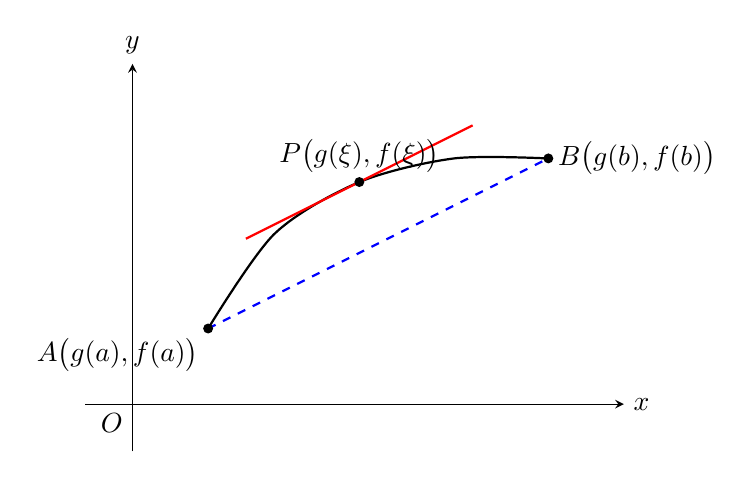
\begin{tikzpicture}[scale=1.2, >=stealth]
            \draw[->] (-0.5,0) -- (5.2,0) node[right] {$x$};
            \draw[->] (0,-0.5) -- (0,3.6) node[above] {$y$};
            \node[below left] at (0,0) {$O$};

            \coordinate (A) at (0.8, 0.8);
            \coordinate (B) at (4.4, 2.6);
            \coordinate (P) at (2.4, 2.35);

            \draw[thick, smooth] plot coordinates {(0.8, 0.8) (1.5, 1.8) (2.4, 2.35) (3.4, 2.6) (4.4, 2.6)};
            \draw[dashed, thick, blue] (A) -- (B);
            \draw[thick, red] (1.2, 1.75) -- (3.6, 2.95);

            \fill (A) circle (1.5pt) node[below left] {$A\bigl(g(a), f(a)\bigr)$};
            \fill (B) circle (1.5pt) node[right] {$B\bigl(g(b), f(b)\bigr)$};
            \fill (P) circle (1.5pt) node[above] {$P\bigl(g(\xi), f(\xi)\bigr)$};
        \end{tikzpicture}
    \end{center}

    连接端点 $A$ 与 $B$ 的割线斜率为
    \begin{equation}
        k_{AB} = \frac{f(b) - f(a)}{g(b) - g(a)}.
    \end{equation}
    在曲线 $C$ 上参数为 $t = \xi$ 的动点 $P\bigl(g(\xi), f(\xi)\bigr)$ 处的切线斜率为
    \begin{equation}
        k_P = \left. \frac{\d y}{\d x} \right|_{t=\xi} = \frac{f'(\xi)}{g'(\xi)}.
    \end{equation}
    Cauchy 中值定理的几何意义为：在满足条件的平面参数曲线弧 $\overparen{AB}$ 上，至少存在一点 $P\bigl(g(\xi), f(\xi)\bigr)$（$\xi \in (a, b)$），使得该点处的切线平行于连接两端点的割线 $AB$．
    \begin{equation}
        \boxed{\text{几何意义：平面参数曲线弧上至少存在一点，该点处的切线平行于两端点的连弦．}}
    \end{equation}
\end{solution}

\begin{problem}{Cauchy 中值定理条件的必要性反例}{Counterexample-To-Cauchy-MVT}
    试说明在闭区间 $[-1, 1]$ 上 Cauchy 中值定理对函数 $f(x) = x^2$ 和 $g(x) = x^3$ 为什么不正确．
\end{problem}

\begin{solution}
    计算端点割线比值：
    \begin{equation}
        \frac{f(1) - f(-1)}{g(1) - g(-1)} = \frac{1 - 1}{1 - (-1)} = \frac{0}{2} = 0.
    \end{equation}
    对任意 $\xi \in (-1, 1)$：
    \begin{enumerate}
        \item 若 $\xi \neq 0$，则导数商为
              \begin{equation}
                  \frac{f'(\xi)}{g'(\xi)} = \frac{2\xi}{3\xi^2} = \frac{2}{3\xi} \neq 0;
              \end{equation}
        \item 若 $\xi = 0$，则 $g'(0) = 0$，导数商 $\frac{f'(0)}{g'(0)}$ 无意义．
    \end{enumerate}
    故在 $(-1, 1)$ 内不存在任何 $\xi$ 使得 $\frac{f(1) - f(-1)}{g(1) - g(-1)} = \frac{f'(\xi)}{g'(\xi)}$．

    原因在于：辅助函数导数 $g'(x) = 3x^2$ 在开区间内部的点 $x = 0 \in (-1, 1)$ 处取零值，违背了 Cauchy 中值定理中“在开区间内 $g'(x) \neq 0$”的先决条件．
    \begin{equation}
        \boxed{\text{原因：函数 } g(x) \text{ 的导数在区间内点 } x = 0 \text{ 处为零，不满足定理条件．}}
    \end{equation}
\end{solution}

\begin{problem}{二次方辅助函数的 Cauchy 中值定理应用}{Cauchy-MVT-Application-Quadratic}
    设 $b > a > 0$，函数 $f(x)$ 在 $[a, b]$ 上连续，在 $(a, b)$ 内可微，求证：存在 $\xi \in (a, b)$，使得
    \begin{equation}
        2\xi\bigl( f(b) - f(a) \bigr) = (b^2 - a^2)f'(\xi).
    \end{equation}
\end{problem}

\begin{myproof}
    令辅助函数 $g(x) = x^2$．

    因为 $b > a > 0$，所以函数 $f(x)$ 与 $g(x)$ 在闭区间 $[a, b]$ 上连续，在开区间 $(a, b)$ 内可导，且对任意 $x \in (a, b)$ 恒有
    \begin{equation}
        g'(x) = 2x > 0 \neq 0.
    \end{equation}
    由 Cauchy 中值定理，在 $(a, b)$ 内至少存在一点 $\xi$，使得
    \begin{equation}
        \frac{f(b) - f(a)}{g(b) - g(a)} = \frac{f'(\xi)}{g'(\xi)} \implies \frac{f(b) - f(a)}{b^2 - a^2} = \frac{f'(\xi)}{2\xi}.
    \end{equation}
    两端交叉相乘，即得
    \begin{equation}
        2\xi\bigl( f(b) - f(a) \bigr) = (b^2 - a^2)f'(\xi).
    \end{equation}
\end{myproof}

\begin{problem}{倒数辅助函数的 Cauchy 中值定理应用}{Cauchy-MVT-Application-Reciprocal}
    设 $f(x)$ 在 $[a, b]$ 上连续（$ab > 0$），在 $(a, b)$ 上可微．求证：存在 $\xi \in (a, b)$，使得
    \begin{equation}
        \frac{af(b) - bf(a)}{a - b} = f(\xi) - \xi f'(\xi).
    \end{equation}
\end{problem}

\begin{myproof}
    令辅助函数
    \begin{equation}
        F(x) = \frac{f(x)}{x}, \qquad G(x) = \frac{1}{x}.
    \end{equation}
    因为 $ab > 0$，所以 $0 \notin [a, b]$，函数 $F(x)$ 与 $G(x)$ 在 $[a, b]$ 上连续，在 $(a, b)$ 内可微．

    求导得
    \begin{equation}
        F'(x) = \frac{x f'(x) - f(x)}{x^2}, \qquad G'(x) = -\frac{1}{x^2} \neq 0.
    \end{equation}
    由 Cauchy 中值定理，在 $(a, b)$ 内至少存在一点 $\xi$，使得
    \begin{equation}
        \frac{F(b) - F(a)}{G(b) - G(a)} = \frac{F'(\xi)}{G'(\xi)}.
    \end{equation}
    展开等式左端：
    \begin{equation}
        \frac{F(b) - F(a)}{G(b) - G(a)} = \frac{\frac{f(b)}{b} - \frac{f(a)}{a}}{\frac{1}{b} - \frac{1}{a}} = \frac{\frac{af(b) - bf(a)}{ab}}{\frac{a - b}{ab}} = \frac{af(b) - bf(a)}{a - b}.
    \end{equation}
    展开等式右端：
    \begin{equation}
        \frac{F'(\xi)}{G'(\xi)} = \frac{\frac{\xi f'(\xi) - f(\xi)}{\xi^2}}{-\frac{1}{\xi^2}} = -\bigl( \xi f'(\xi) - f(\xi) \bigr) = f(\xi) - \xi f'(\xi).
    \end{equation}
    因此
    \begin{equation}
        \frac{af(b) - bf(a)}{a - b} = f(\xi) - \xi f'(\xi).
    \end{equation}
\end{myproof}

\endinput
